\section{Routing Layer Design\label{sec:routing}}
Routing transactions between different blockchains remains a difficult problem. Natively, blockchains have no concept of networking, DNS or other temporal data; and storing these on-chain is both prohibitively expensive, as well as a bad idea, as temporary network outages must not cause consensus failure. To accommodate for the limitations of blockchains, we are developing a network of decentralized nodes to provide oracle and relaying services, based on crypto-economic security primitives and threshold-signature-sharing. Staking and fee incentives secure the network and ensure longevity. By cleverly combining these services, we are capable of executing protocol-to-protocol interactions across chains. In the cross-chain, cross-layer scenario we operate, it is crucial to find the best route to exploit. A good route can reduce the time of transactions, the associated costs and minimize the risks taken by the user. Hence, the routing layer design directly affects the quality of our service and the user experience. 

Our routing layer solves two problems: constructing and maintaining a graph of the different chains and bridges available, and, finding the best route at a given time. With the increasing number of chains (both on Layer 1 and Layer 2), and the different available bridge solutions between them, maintaining a live graph of all the connections is not a trivial task. In a dense graph, the number of edges connecting the vertices grows quadratically. We also need to consider the mutating and changing nature of blockchain ecosystems: new versions of protocols can be deployed, old bridges might drop support, new tokens can be added etc. 

Given the magnitude and dynamic essence of the task, and the volatile prices we face, finding the optimal route for a given trade is not in the reach of most of the users. The problem can be seen as an instance of the Travelling salesman problem \cite{Gavish1978TheProblems} or the Minimum-cost flow problem \cite{Orlin1988AAlgorithm}, with the component of changing networks and the requirement of on-chain validity. The users need to be guaranteed they got the best possible path. In order to accomplish all this, we require complex algorithms (e.g: \cite{Feigenbaum2005ARouting}) and dedicated heuristics.

One exciting application for this execution layer is in cross-chain fee management. Our infrastructure as a whole intends to support a network of blockchain networks, meaning that there will be multiple potential pathways to the same destination. In this scenario, without a tool to do so for them, users would have to pathfind the most efficient and compliant route for value packets. Users may need to prioritize efficiency if the pathway must be especially liquid or secure, or if a specific regulatory requirement must be enforced (such as know your customer/anti-money laundering requirements, abbreviated KYC/AML). Therefore, the routing process would be both incredibly important and very time intensive. Our pathway execution layer will make this process simple for users and enable them to customize which parameter they want to optimize for when completing a given transaction.

Our routing layer will abstract and simplify the route algorithms through a clean and straightforward interface. In an effort to decentralize our solution and increase the transparency of DeFi projects, we also plan to include the following services and parties within our solution.

\subsection{Nameservices}
A nameservice is a simple registry that maps identifications to names (e.g: DNS). This feature can also be used to link blockchain addresses to names (e.g: nicknames). Nameservices improve the semantic meaning of decentralized protocols, help the inexperienced user, bridge different platforms, decrease the possibility of making errors when creating transactions and contribute to promote identity and digital ownership on Web3.

While other projects have already explored the benefits of using nameservices \cite{ProtonchainBlockchain}. To the best of our knowledge, Composable Finance will be the first one to provide cross-chain and cross-layer nameservice support. Providing nameservice support on a single chain is relatively trivial. However, maintaining nameservices across different layers and chains poses new challenges. We will take care of the details such as key management, data synchronization and finality on different chains so that the whole process is translucent to the final user. Therefore, no matter the network or the token, we will be able to support names and addresses indistinctly.

Nameservices help to accomplish our vision of a less fragmented and more accessible blockchain space. Where a single interface helps to leverage the composability of the DeFi space, unlocking its full potential and enabling new projects.

\subsection{Indexers and Solvers}
As mentioned beforehand, constructing a dynamic graph and finding the best route within it, are the main challenges our routing layer faces. In achieving these goals, we also want to ensure the decentralization and auditability of the solution. For this reason, we introduce two parties, which can be run by anyone, that will have a crucial role on the protocol:

\begin{itemize}
    \item Indexers will act as oracles and will help to update the graph of interconnected chains and bridges. Every time there is a change on the topology of the network (new bridges/chains, network disruptions, significant changes on costs, etc.), indexers will notify it. Indexers notifications will be weighted and taken into account to update the main graph. Indexers will obtain rewards in rewards in function of the utility of the updates and a slashing mechanism will be used to prevent malicious indexers.
    
    \item Solvers will run off-chain custom algorithms to find the best route for a given problem instance. When trying to find a path, solvers will compete to find the best solution. Received solutions will be ranked according to a predefined cost function and top solvers will earn tokens with regard to the efficiency of their solution. By doing this, we leverage the game theory aspect of the competition while achieving a decentralized manner to find the best route.
    
\end{itemize}

\begin{figure}[h]
    \centering
    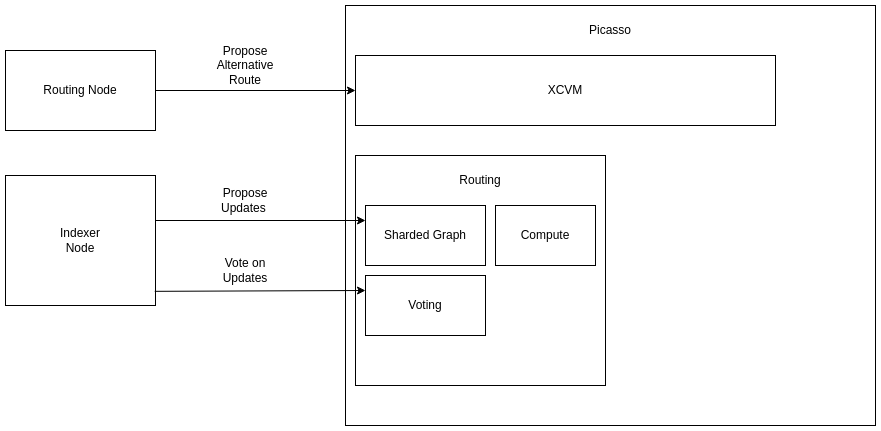
\includegraphics[width=0.85\textwidth]{images/routing.png}
    \caption{Routing architecture with indexers and solvers. We can appreciate how, by using Picasso as finality layer, routers and indexers can collaborate on the routing algorithm. Please note how routing solver nodes leverage XCVM to propose new routes.}
    \label{fig:routing}
\end{figure}

These roles will be used, together with a default minimum cost routing algorithm, to address the routing challenges previously introduced. This architecture, as shown in Figure \ref{fig:routing}, enhances for public examination and minimizes the trust users need to put on the protocol. It is also fairly easy to scale since most of the workload is performed off-chain, while only validation is done on-chain.

\begin{figure}[ht]
    \centering
    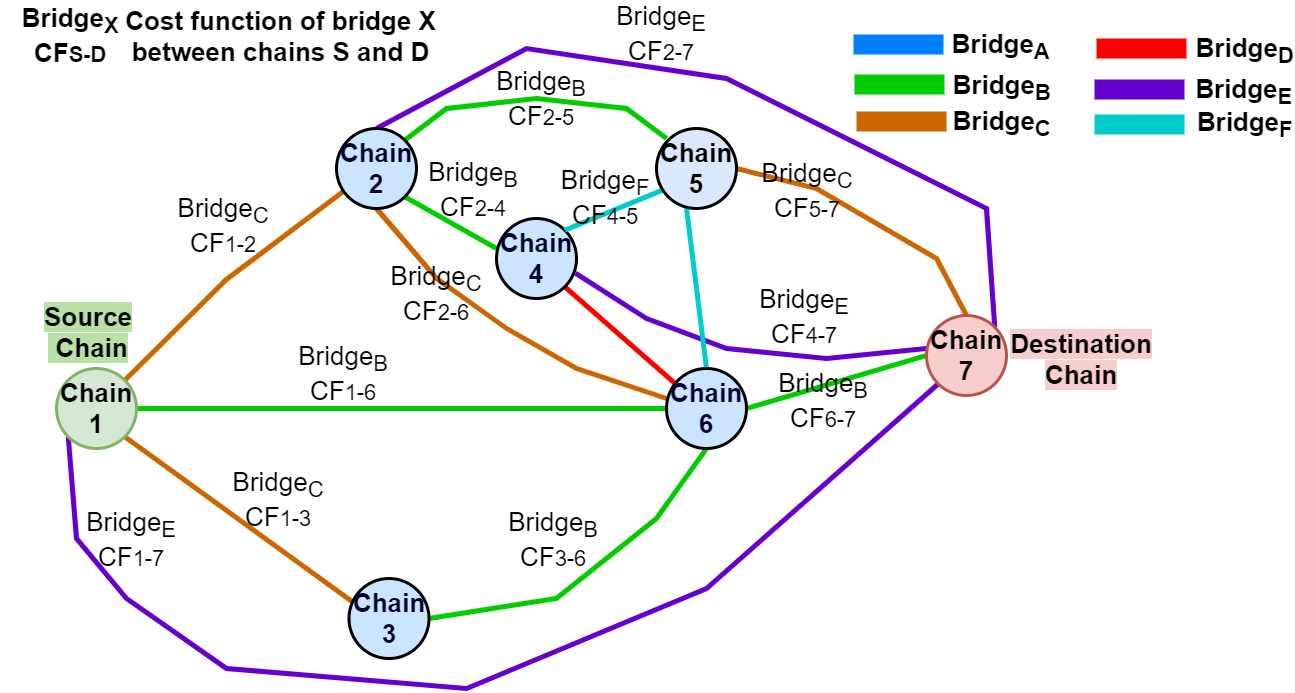
\includegraphics[width=0.85\textwidth]{images/Selected_Bridges1.png}
    \caption{Uni-connected directional graph representation of different Blockchains connected via the best bridges based on the specific requirements of a given user at a given time.}
    \label{fig:sel_bridges}
\end{figure}

As for the routing algorithms employed by solvers, we do not enforce any kind of restriction. We are interested on the best result the community can provide. As previously mentioned, and shown in Figure \ref{fig:sel_bridges}, we are facing a complex problem with variable parameters, where there is no unique strategy that dominates the others, at least with limited time. We outsource the path finding task to the decentralized community of Composable users. As other projects have explored \cite{GnosisWhitepaper}, having the users to run different algorithms and heuristics in a fair ecnonomic game, produces a better and more complete solution that can adapt to new scenenarios faster. We will also run our own algorithm, so that all problem instances have a fair baseline solution.